\section{Preliminaries}
Evaluation of SQL queries over incomplete databases is a well known problem since 1970(s), however people commonly say "You can never trust the answers you get from a database with nulls." \cite{date2005database}. 
Indeed, the way SQL handle incomplete information still produce counter-intuitive and just plain incorrect answers.

\subsection{SQL behavior}
\begin{figure}[h]
	\caption{\label{db} SQL Database}
	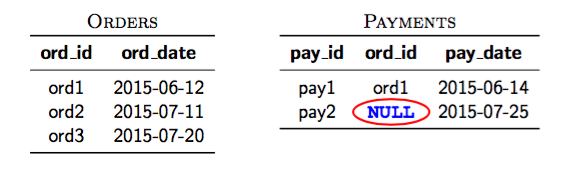
\includegraphics[scale=0.5]{query1}
\end{figure}

\begin{figure}[h]
	\caption{\label{query} SQL Query}
\begin{lstlisting}[language=SQL]
SELECT ord_id FROM Orders 
WHERE NOT EXISTS  
	(SELECT * FROM Payments WHERE Payments.ord_id = Orders.ord_id)
\end{lstlisting}
\end{figure}



When we evaluate the query \ref{query} on the database \ref{db} we obtain $\llbracket ord2,ord3\rrbracket$. However this answer does not fit the notion of correctness, indeed $NULL$ can be interpret as $ord2$ or $ord3$, meaning that none of them is a correct answer. 

Such "false-positive" answers occur in real life queries \cite{guagliardo2016making}. Then it is natural to find a way to prevent them.  


%It is important to notice that our evaluation algorithm can easily be adapt in order to return a set containing all certain-answers, ie. an over-approximation.








